\documentclass[a4paper,12pt,oneside]{book}
\usepackage[utf8]{inputenc}
\usepackage{amssymb}
\usepackage{amsmath}
\usepackage{graphicx}
\graphicspath{ {images/} }
\usepackage{times}
\usepackage{geometry}
\usepackage{setspace}
\usepackage{tocloft}
\usepackage{tabu}
\usepackage{fancyhdr}
\geometry{a4paper, tmargin=1in, rmargin=1in, bmargin=1in, lmargin=1.5in}


%-----------------------------------------
% Editables of the document
%-----------------------------------------
\newcommand{\thesistitle}{Secure Data Transmission over Cloud Computing using Improved Block Chain Technology with CRT-RSA} % Title of the Thesis, change here
\newcommand{\thesisauthora}{K.Rithanya Sai  (1601-21-778-001)} % Person 1-
\newcommand{\thesisauthorb}{K.Monish Viswak (1601-21-778-002)} % Person 2-
\newcommand{\thesisauthorc}{K.Devaansh (1601-21-778-003)} % Person 3-
% If the number of people is different, change accordingly in titlepage and bonafide -certificate
\newcommand{\thesisdept}{Artificial Intelligence and Data Science} % Department
\newcommand{\thesisguide}{Dr.Satya Kiranmai Tadepalli} % Project Guide
\newcommand{\depthod}{Prof.K.Radhika} % Department Head
% Also, change the graduation year in titlepage and bonafide certificate
%-----------------------------------------

% References are to be added in reference.bib and cited in any part of the document. Read any examples online on how to add references. You can also use Google Scholar to get the reference formatted for BibTex.


% For Figures and Subfigures
\usepackage{graphicx, caption, subcaption}

% Package for block commenting
\usepackage{comment}

\usepackage{physics}

% Package to keep images in place
\usepackage{float}

% Package for Appendices
\usepackage{titletoc}
\usepackage{appendix}

% Chapter and Appendix in TOC prefixed
\makeatletter
\titlecontents{chapter}%
 [0pt]% 
 {\bfseries}%
 {\MakeUppercase \@chapapp\ \thecontentslabel\quad}% 
 {}% 
 {\normalfont\cftdotfill{\cftdotsep}\contentspage}% 
 [\addvspace{0pt}]% 

\g@addto@macro\appendices{%
  \addtocontents{toc}{\protect\renewcommand{\protect\@chapapp}{\appendixname}}%
}
\makeatother


% Package for codes
\usepackage{listings}
\lstset{
    breaklines = true,
    captionpos = b,
    numberstyle = \scriptsize,
    numbers=left,                    
    numbersep=10pt
}


% Package for enumerate
\usepackage{enumitem}

% Block Diagram Packages and Functions
\usepackage{tikz}
\usetikzlibrary{arrows, decorations.markings}
\usetikzlibrary{arrows,positioning,shapes.geometric}
\tikzstyle{vecArrow} = [thick, decoration={markings,mark=at position
   1 with {\arrow[semithick]{open triangle 60}}},
   double distance=1.4pt, shorten >= 5.5pt,
   preaction = {decorate},
   postaction = {draw,line width=1.4pt, white,shorten >= 4.5pt}]
\tikzstyle{innerWhite} = [semithick, white,line width=1.4pt, shorten >= 4.5pt]
\tikzstyle{block} = [draw, fill=blue!20, rectangle, 
    minimum height=3em, minimum width=6em]

% Chapter Title Customization
\usepackage{titlesec}
%\titleformat{\chapter}[display]% OLD
%    {\normalfont\huge\bfseries}{\chaptertitlename\ \thechapter}{20pt}{\Huge}% OLD
% \titlespacing*{\chapter}{0pt}{50pt}{40pt}% OLD

\titleformat{\chapter}[display]
{\Large\bfseries\centering}{\MakeUppercase\chaptertitlename\ \thechapter}{5pt}{\Large}
\titlespacing*{\chapter}{0pt}{0pt}{20pt}

% Section Customization
\titleformat{\section}{\large \bfseries}{\thesection}{1em}{}

% Sub-Section Customization
\titleformat{\subsection}{\fontsize{13pt}{13pt} \bfseries}{\thesubsection}{1em}{}


% Align the titles of auxiliary content to center
\renewcommand*\contentsname{\Large \centerline{TABLE OF CONTENTS}}
\renewcommand*\listfigurename{\Large \centerline{LIST OF FIGURES}}
\renewcommand*\listtablename{\Large \centerline{LIST OF TABLES}}


% References Addition
\usepackage[backend=bibtex,
style=numeric,
bibencoding=ascii,
maxbibnames=99,
sorting=none
%style=alphabetic
%style=reading
]{biblatex}
\addbibresource{reference.bib}

% Page Style
\pagestyle{fancy}
\cfoot{\thepage}
\rhead{}
\lhead{}
\renewcommand{\headrulewidth}{0pt}
\renewcommand{\footrulewidth}{0pt}

% Line Spacing
\usepackage{setspace}

% Indent First Paragraph
\usepackage{indentfirst}

% To make uppercase words
\usepackage{textcase}


\usepackage[bookmarks, colorlinks=false, pdfborder={0 0 0}, pdftitle={\thesistitle}, pdfkeywords={}]{hyperref}


\begin{document}

% To expand the word spacing
\spaceskip=1.5\fontdimen2\font plus 1.5\fontdimen3\font
minus 1.5\fontdimen4\font


\frontmatter
\pagenumbering{gobble}
\begin{titlepage}
\begin{center}
\fontsize{20pt}{1cm}\selectfont \textbf{\thesistitle}

\vspace*{0.8cm}
\fontsize{14pt}{21pt}\selectfont A Mini Project Report \\
submitted in partial fulfillment of the requirements for \\
the award of the degree of

\vspace*{0.3cm}
\fontsize{14pt}{1cm}\selectfont\textbf{Bachelor of Engineering} 

\vspace*{0.3cm}
\textbf{in\\\thesisdept}

\vspace*{0.5cm}
By

\textbf{\thesisauthora}\\
\textbf{\thesisauthorb}\\
\textbf{\thesisauthorc}\\
\vspace*{0.5cm}
\textbf{\textit{Under the esteemed guidance of}}\\
\textbf{Dr. Satya Kiranmai Tadepalli}\\
Assistant Professor\\
\vfill

\includegraphics[width=1.25in]{cbit.png}

\vspace*{0.3in}
\fontsize{12pt}{12pt}\selectfont \textbf{DEPARTMENT OF ARTIFICIAL INTELLIGENCE AND DATA SCIENCE}\\[0.2cm]
\fontsize{14pt}{14pt}\selectfont\textbf{CHAITANYA BHARATHI INSTITUTE OF TECHNOLOGY}\\[0.2cm]
\textbf{HYDERABAD -- 500075}

\vspace*{0.2cm}
\textbf{NOVEMBER 2026}
\end{center}
\end{titlepage}
\thispagestyle{empty}
%\begin{center}
%\textbf{BONAFIDE CERTIFICATE}
%\end{center}
\begin{center}

\includegraphics[width=1.0in]{cbit.png}

\vspace*{0.3in}
\fontsize{12pt}{12pt}\selectfont \textbf{DEPARTMENT OF ARTIFICIAL INTELLIGENCE AND DATA SCIENCE}\\[0.2cm]
\fontsize{14pt}{14pt}\selectfont\textbf{CHAITANYA BHARATHI INSTITUTE OF TECHNOLOGY}\\[0.2cm]
\textbf{HYDERABAD -- 500075}\\
\vspace*{0.3in}
\fontsize{16pt}{16pt}\textbf{INSTITUTE VISION}
\end{center}


\vspace{0.05cm}
\noindent
\fontsize{10pt}{24pt}\selectfont “To be the center of excellence in technical education and research”.


\begin{center}
\fontsize{16pt}{16pt}\textbf{INSTITUTE MISSION}
\end{center}

\vspace{0.05cm}
\noindent
\fontsize{10pt}{24pt}\selectfont “To address the emerging needs through quality technical education and advanced research”.

\vspace{0.05cm}

\begin{center}
\fontsize{16pt}{16pt}\textbf{DEPARTMENT VISION}
\end{center}

\vspace{0.05cm}
\noindent
\fontsize{10pt}{24pt}\selectfont "To be a globally recognized center of excellence in the field of Artificial Intelligence and Data Science that produces innovative pioneers and research experts capable of addressing complex real-world challenges and contributing to the socio-economic development of the nation."

\begin{center}
\fontsize{16pt}{16pt}\textbf{DEPARTMENT MISSION}
\end{center}
 
\vspace{0.05cm}
\noindent
\fontsize{10pt}{24pt}\selectfont
\begin{enumerate}
    \item To provide cutting-edge education in the field of Artificial Intelligence and Data Science that is rooted in ethical and moral values.
    \item To establish strong partnerships with industries and research organizations in the field of Artificial Intelligence and Data Science, and to excel in the emerging areas of research by creating innovative solutions.
    \item To cultivate a strong sense of social responsibility among students, fostering their inclination to utilize their knowledge and skills for the betterment of society.
    \item To motivate and mentor students to become trailblazers in Artificial Intelligence and Data Science, and develop an entrepreneurial mindset that nurtures innovation and creativity.
\end{enumerate}



\newpage
\thispagestyle{empty}
%\begin{center}
%\textbf{BONAFIDE CERTIFICATE}
%\end{center}
\begin{center}

\includegraphics[width=1.0in]{cbit.png}

\vspace*{0.3in}
\fontsize{12pt}{12pt}\selectfont \textbf{DEPARTMENT OF ARTIFICIAL INTELLIGENCE AND DATA SCIENCE}\\[0.2cm]
\fontsize{14pt}{14pt}\selectfont\textbf{CHAITANYA BHARATHI INSTITUTE OF TECHNOLOGY}\\[0.2cm]
\textbf{HYDERABAD -- 500075}\\
\vspace*{0.3in}
\fontsize{16pt}{16pt}\textbf{PROGRAM EDUCATIONAL OBJECTIVES (PEOs)}
\end{center}


\vspace{0.05cm}
\noindent
\fontsize{10pt}{24pt}\selectfont Graduates of AI \& DS will be able to:
\begin{enumerate}
    \item Adapt emerging technologies of Artificial Intelligence \& Data Science and develop state of the art solutions in the fields of Manufacturing, Agriculture, Health-care, Education, and Cyber Security.
    \item Exhibit professional leadership qualities to excel in interdisciplinary domains.
    \item Possess human values, professional ethics, application-oriented skills, and engage in lifelong learning.
    \item Contribute to the research community to meet the needs of public and private sectors.
\end{enumerate}

\begin{center}
\fontsize{16pt}{16pt}\textbf{PROGRAM SPECIFIC OUTCOMES (PSOs)}
\end{center}

\vspace{0.05cm}
\noindent
\fontsize{10pt}{24pt}\selectfont After successful completion of the program, students will be able to:
\vspace{0.05cm}
\begin{enumerate}
    \item Exhibit proficiency of Artificial Intelligence and Data Science in providing sustainable solutions by adapting to societal, environmental and ethical concerns to real world problems.
    \item Develop professional skills in the thrust areas like ANN and Deep learning, Robotics, Internet of Things and Big Data Analytics.
    \item Pursue higher studies in Artificial Intelligence and Data Science in reputed Universities and to work in research establishments.

\end{enumerate}



\newpage
\thispagestyle{empty}
%\begin{center}
%\textbf{BONAFIDE CERTIFICATE}
%\end{center}
\begin{center}

\includegraphics[width=1.0in]{cbit.png}

\vspace*{0.3in}
\fontsize{12pt}{12pt}\selectfont \textbf{DEPARTMENT OF ARTIFICIAL INTELLIGENCE AND DATA SCIENCE}\\[0.2cm]
\fontsize{14pt}{14pt}\selectfont\textbf{CHAITANYA BHARATHI INSTITUTE OF TECHNOLOGY}\\[0.2cm]
\textbf{HYDERABAD -- 500075}\\
\vspace*{0.3in}
\fontsize{16pt}{16pt}\textbf{PROGRAM OUTCOMES}
\end{center}


\vspace{0.05cm}
\noindent
\fontsize{10pt}{24pt}\selectfont 
\begin{enumerate}
    \item \textbf{Engineering Knowledge:} Apply knowledge of mathematics, natural science, computing, engineering fundamentals and an engineering specialization as specified in WK1 to WK4 respectively to develop to the solution of complex engineering problems.
    \item \textbf{Problem Analysis:} Identify, formulate, review research literature and analyze complex engineering problems reaching substantiated conclusions with consideration for sustainable development. (WK1 to WK4)
    \item \textbf{Design/Development of Solutions:} Design creative solutions for complex engineering problems and design/develop systems/components/processes to meet identified needs with consideration for the public health and safety, whole-life cost, net zero carbon, culture, society and environment as required. (WK5)
    \item \textbf{Conduct Investigations of Complex Problems:} Conduct investigations of complex engineering problems using research-based knowledge including design of experiments, modelling, analysis \& interpretation of data to provide valid conclusions. (WK8).
    \item \textbf{Engineering Tool Usage:} Create, select and apply appropriate techniques, resources and modern engineering \& IT tools, including prediction and modelling recognizing their limitations to solve complex engineering problems. (WK2 and WK6)
    \item \textbf{The Engineer and The World:} Analyze and evaluate societal and environmental aspects while solving complex engineering problems for its impact on sustainability with reference to economy, health, safety, legal framework, culture and environment. (WK1, WK5, and WK7).
    \item \textbf{Ethics:} Apply ethical principles and commit to professional ethics, human values, diversity and inclusion; adhere to national \& international laws. (WK9)
    \item \textbf{Individual and Collaborative Team work:} Function effectively as an individual, and as a member or leader in diverse/multi-disciplinary teams.
    \item \textbf{Communication:} Communicate effectively and inclusively within the engineering community and society at large, such as being able to comprehend and write effective reports and design documentation, make effective presentations considering cultural, language, and learning differences
    \item \textbf{Project Management and Finance:} Apply knowledge and understanding of engineering management principles and economic decision-making and apply these to one’s own work, as a member and leader in a team, and to manage projects and in multidisciplinary environments.
    \item \textbf{Life-Long Learning:} Recognize the need for, and have the preparation and ability for i) independent and life-long learning ii) adaptability to new and emerging technologies and iii) critical thinking in the broadest context of technological change. (WK8)


\end{enumerate}





\newpage
\thispagestyle{empty}
%\begin{center}
%\textbf{BONAFIDE CERTIFICATE}
%\end{center}
\begin{center}

\includegraphics[width=1.0in]{cbit.png}

\vspace*{0.3in}
\fontsize{12pt}{12pt}\selectfont \textbf{DEPARTMENT OF ARTIFICIAL INTELLIGENCE AND DATA SCIENCE}\\[0.2cm]
\fontsize{14pt}{14pt}\selectfont\textbf{CHAITANYA BHARATHI INSTITUTE OF TECHNOLOGY}\\[0.2cm]
\textbf{HYDERABAD -- 500075}\\
\vspace*{0.3in}
\fontsize{16pt}{16pt}\textbf{\underline{MINI PROJECT-II}}
\end{center}

\begin{center}

\fontsize{16pt}{16pt}\textbf{COURSE OBJECTIVES}
\end{center}
\noindent
\fontsize{10pt}{24pt}\selectfont 
\begin{enumerate}[noitemsep]
    \item To enable students learning by doing.
    \item To develop capability to analyse and solve real world problems.
    \item To inculcate innovative ideas of the students.
    \item To impart team building and management skills among students.
    \item To instill writing and presentation skills for completing the project.
\end{enumerate}

\begin{center}

\fontsize{16pt}{16pt}\textbf{COURSE OUTCOMES}
\end{center}


\vspace{0.05cm}
\noindent
\fontsize{10pt}{24pt}\selectfont Upon successful completion of this course, students will be able to:
\begin{enumerate}[noitemsep]
    \item Interpret Literature with the purpose of formulating a project proposal.
    \item Plan, Analyse, Design and Implement a project.
    \item Find the solution of identified problem with the help of modern Technology and give priority to real time scenarios.
    \item Plan to work as a team and to focus on getting a working project done and submit a report within a stipulated period of time.
    \item Prepare and submit the Report and deliver presentation before the Departmental Committee.
\end{enumerate}



\newpage
\thispagestyle{empty}
%\begin{center}
%\textbf{BONAFIDE CERTIFICATE}
%\end{center}
\begin{center}

\includegraphics[width=1.0in]{cbit.png}

\vspace*{0.3in}
\fontsize{12pt}{12pt}\selectfont \textbf{DEPARTMENT OF ARTIFICIAL INTELLIGENCE AND DATA SCIENCE}\\[0.2cm]
\fontsize{14pt}{14pt}\selectfont\textbf{CHAITANYA BHARATHI INSTITUTE OF TECHNOLOGY}\\[0.2cm]
\textbf{HYDERABAD -- 500075}\\
\vspace*{0.3in}
\fontsize{16pt}{16pt}\textbf{\underline{CO-PO MAPPING}}
\end{center}

\begin{table}[H]
    \centering
        \begin{tabular}{|c|c|c|c|c|c|c|c|c|c|c|c|c|}
        \hline
         &PO1&PO2&PO3&PO4&PO5&PO6&PO7&PO8&PO9&PO10&PO11\\
        \hline
        CO1 &3& 3& 2& 3& 3& 3& 2& 1& 2& 3& 3 \\
        \hline
        CO2 &3 &3 &3 &3 &3 &3 &2 &1 &2 &3 &3 \\
        \hline
        CO3 &3 &3 &3 &3 &3 &3 &2 &- &2 &3 &3 \\
        \hline
        CO4 &2 &2 &2 &3 &3 &3 &2 &3 &3 &2 &3 \\
        \hline
        CO5 &1 &2 &1 &2 &3 &3 &- &2 &3 &- &- \\
        \hline
        \end{tabular}
    \caption*{Mapping of Course Outcomes with Program Outcomes}
\end{table}

\begin{center}
\fontsize{16pt}{16pt}\textbf{\underline{CO-PSO MAPPING}}
\end{center}

\begin{table}[H]
    \centering
        \begin{tabular}{|c|c|c|c|}
        \hline
         &PSO1&PSO2&PSO3\\
        \hline
        CO1 & 2& 3& 2 \\
        \hline
        CO2 &1 &3 &2\\
        \hline
        CO3 &3 &3 &2\\
        \hline
        CO4 &2 &3 &2\\
        \hline
        CO5 &2 &3 &-\\
        \hline
        \end{tabular}
    \caption*{Mapping of Course Outcomes with Program Specific Outcomes}
\end{table}


\newpage
\thispagestyle{empty}

\begin{center}

\includegraphics[width=1.25in]{cbit.png}

\vspace*{0.3in}
\fontsize{12pt}{12pt}\selectfont \textbf{DEPARTMENT OF ARTIFICIAL INTELLIGENCE AND DATA SCIENCE}\\[0.2cm]
\fontsize{14pt}{14pt}\selectfont\textbf{CHAITANYA BHARATHI INSTITUTE OF TECHNOLOGY}\\[0.2cm]
\textbf{HYDERABAD -- 500075}\\
\vspace*{0.3in}
%\begin{center}
\fontsize{16pt}{16pt}\textbf{DECLARATION CERTIFICATE}
%\end{center}
\end{center}

%\chapter*{DECLARATION CERTIFICATE}

\vspace{0.3cm}
\noindent
\fontsize{12pt}{24pt}\selectfont 

We hereby declare that the mini project titled \textbf{\thesistitle} submitted by us to the  \textbf{\thesisdept} \textbf{CHAITANYA BHARATHI INSTITUTE OF TECHNOLOGY, HYDERABAD} in partial fulfillment of the requirements for the award of \textbf{Bachelor of Engineering} is a bona-fide record of the work carried out by us under the supervision of \textbf{Dr. Kadiyala Ramana}  .
We further declare that the work reported in this project, has not been submitted
and will not be submitted, either in part or in full, for the award of any other degree or
diploma of this institute or of any other institute or University.





\vspace{2.5cm}



{\raggedleft Project Associates\\
\textbf{\thesisauthora}\\
\textbf{\thesisauthorb}\\
\textbf{\thesisauthorc}\\
}



\newpage
\thispagestyle{empty}
%\begin{center}
%\textbf{BONAFIDE CERTIFICATE}
%\end{center}
\begin{center}

\includegraphics[width=1.0in]{cbit.png}

\vspace*{0.3in}
\fontsize{12pt}{12pt}\selectfont \textbf{DEPARTMENT OF ARTIFICIAL INTELLIGENCE AND DATA SCIENCE}\\[0.2cm]
\fontsize{14pt}{14pt}\selectfont\textbf{CHAITANYA BHARATHI INSTITUTE OF TECHNOLOGY}\\[0.2cm]
\textbf{HYDERABAD -- 500075}\\
\vspace*{0.3in}
\fontsize{16pt}{16pt}\textbf{BONAFIDE CERTIFICATE}
\end{center}
%\chapter*{BONAFIDE CERTIFICATE}

\vspace{0.15cm}
\noindent
\fontsize{12pt}{24pt}\selectfont This is to certify that the project titled \textbf{\thesistitle} is a bonafide record of the work done by
%\vspace{0.1cm}

\begin{center}
\textbf{\thesisauthora}\\
\textbf{\thesisauthorb}\\
\textbf{\thesisauthorc}\\
\end{center}

\vspace{0.05cm}
\noindent
\fontsize{12pt}{24pt}\selectfont in partial fulfillment of the requirements for the award of the degree of \textbf{Bachelor of Engineering} in \textbf{\thesisdept} to the \textbf{CHAITANYA BHARATHI INSTITUTE OF TECHNOLOGY, HYDERABAD} carried out under my guidance and supervision during the year 2026-27. The results presented in this project report have not been submitted to any other university or Institute for the
award of any degree.
 


\vspace{1.3cm}

\noindent
\begin{tabular*}{\textwidth}{@{} c @{\extracolsep{\fill}} c @{}}
    \textbf{\thesisguide} & \textbf{\depthod}\\
    Guide & Head of the Department
\end{tabular*}

\vspace{1.5cm}

\noindent
Submitted for Semester Mini-Project viva-voce examination held on \underline{\hspace{3cm}}

\vspace{1cm}
\noindent
\textbf{Examiner-1} \hfill \textbf{Examiner-2}

\newpage


\clearpage
\pagenumbering{roman}
\fontsize{12pt}{12pt}\selectfont
\onehalfspacing
\addtocontents{toc}{\textbf{Title}\hfill\textbf{Page No.}\par}
\clearpage
\phantomsection
\addcontentsline{toc}{chapter}{ABSTRACT}
\chapter*{ABSTRACT}
Lorem ipsum dolor sit amet, consectetur adipiscing elit. Curabitur pretium ac ante et sollicitudin. Ut aliquam diam sit amet aliquet viverra. Aliquam erat volutpat. Quisque aliquam pellentesque magna, eget dignissim sem fringilla id. Suspendisse feugiat nisl in consectetur luctus. In hac habitasse platea dictumst. Mauris quis metus eget neque faucibus vestibulum. Proin auctor malesuada felis, at tempus mauris vehicula ac. Donec mauris ex, facilisis eu ullamcorper quis, laoreet vitae sapien. Nunc eget blandit libero. Nulla facilisi.

Lorem ipsum dolor sit amet, consectetur adipiscing elit. Curabitur pretium ac ante et sollicitudin. Ut aliquam diam sit amet aliquet viverra. Aliquam erat volutpat. Quisque aliquam pellentesque magna, eget dignissim sem fringilla id. Suspendisse feugiat nisl in consectetur luctus. In hac habitasse platea dictumst. Mauris quis metus eget neque faucibus vestibulum. Proin auctor malesuada felis, at tempus mauris vehicula ac. Donec mauris ex, facilisis eu ullamcorper quis, laoreet vitae sapien. Nunc eget blandit libero. Nulla facilisi.
\\

\textit{Keywords} : Keyword1, Keyword2, 
\clearpage
\phantomsection
\addcontentsline{toc}{chapter}{ACKNOWLEDGEMENTS}
\chapter*{ACKNOWLEDGEMENTS}


\noindent
\fontsize{12pt}{18pt}\selectfont We take this opportunity to express our deepest gratitude to all those who guided and supported us throughout this course. Without them, this project and the results achieved from it would not have been possible.

\noindent
We are sincerely grateful to \textbf{Sri N.Subash}, President, Chaitanya Bharathi Institute of Technology, Hyderabad for providing an environment that encourages learning, research and innovation.

\noindent
We extend our heartfelt thanks to \textbf{Dr. C.Venkata Narasimhulu}, Principal, Chaitanya Bharathi Institute of Technology, Hyderabad, for the constant encouragement and for providing the infrastructure and resources needed to carry out this project.

\noindent
We are thankful to \textbf{\depthod}, Head of the Department, Department of \thesisdept, for permitting us to make use of the department's facilities and for the support extended throughout our work.

\noindent
We owe a special debt of gratitude to our guide, \textbf{\thesisguide}, Associate Professor, Department of \thesisdept, for the valuable guidance, insightful suggestions and continuous support offered at every stage of this project. This work could not have been completed successfully without that guidance, and the patience and genial attitude shown to us will always remain a source of inspiration.

\noindent
We also thank the faculty and staff members of the Department of \thesisdept for their cooperation and assistance. Finally, we are grateful to our parents and friends for their constant encouragement, support and understanding throughout this journey.

% Table of Contents Page
\clearpage
\phantomsection
\doublespacing
\addcontentsline{toc}{chapter}{TABLE OF CONTENTS}
\tableofcontents

% List of Tables Page
\clearpage
\phantomsection
\doublespacing
\addcontentsline{toc}{chapter}{LIST OF TABLES}
\listoftables

% List of Figures Page
\clearpage
\phantomsection
\doublespacing
\addcontentsline{toc}{chapter}{LIST OF FIGURES}
\listoffigures


% Main Content
\mainmatter
\onehalfspacing
\fancyhead[L]{\textbf{The performance of new graduates}}
\fancyfoot[R]{\textbf{Dept. of AI\&DS, CBIT, Hyderabad}}
\chapter{INTRODUCTION}

Lorem ipsum\cite{loremipsum} dolor sit amet, consectetur adipiscing elit. Etiam consectetur libero dui, sit amet rutrum lectus mollis ac. Phasellus mattis augue quis auctor ullamcorper. Sed congue rutrum turpis, sit amet tincidunt erat laoreet ac. Morbi in feugiat erat, sit amet placerat lorem. Quisque cursus gravida nulla, nec pulvinar justo rutrum eget. Aenean et dolor vitae enim congue maximus. Praesent consequat finibus imperdiet. Sed ipsum erat, efficitur vitae urna a, convallis ornare ipsum. Quisque fringilla risus enim, ut elementum dui consectetur eu.

\section{A Section}

Lorem ipsum\cite{loremipsum} dolor sit amet, consectetur adipiscing elit. Etiam consectetur libero dui, sit amet rutrum lectus mollis ac. Phasellus mattis augue quis auctor ullamcorper. Sed congue rutrum turpis, sit amet tincidunt erat laoreet ac. Morbi in feugiat erat, sit amet placerat lorem. Quisque cursus gravida nulla, nec pulvinar justo rutrum eget. Aenean et dolor vitae enim congue maximus. Praesent consequat finibus imperdiet. Sed ipsum erat, efficitur vitae urna a, convallis ornare ipsum. Quisque fringilla risus enim, ut elementum dui consectetur eu.

\subsection{Part of a section}

Vivamus sed enim quam. In facilisis consequat eros, id convallis diam congue et. Vivamus sed neque rutrum, gravida urna non, lobortis leo. Curabitur sagittis turpis sit amet dolor blandit lobortis. Fusce ac sem eget libero semper ultrices. Aliquam erat volutpat. Quisque tincidunt mi sapien, eu varius libero lacinia quis. Nullam dictum quam sed scelerisque aliquet. Mauris laoreet est nec dolor pellentesque dignissim. Praesent ac sapien erat. Mauris ut felis sit amet velit convallis cursus quis a tellus. Curabitur efficitur ultricies dui, eget vestibulum arcu venenatis ac. Nulla fermentum dolor a venenatis posuere. Vivamus eu luctus erat.\\

Here is a table attached :
\begin{table}[H]
    \centering
        \begin{tabular}{|c|c|}
        \hline
        $n$ & $F_n$\\
        \hline
        1 & 1 \\
        \hline
        2 & 1 \\
        \hline
        3 & 2 \\
        \hline
        4 & 3 \\
        \hline
        \end{tabular}
    \caption{Fibonacci Table}
\end{table}

Morbi pulvinar turpis at ligula sollicitudin, et finibus nulla vestibulum. Etiam molestie tincidunt molestie. Mauris augue ex, tincidunt non ante eget, ultrices ornare quam. Nulla pellentesque fringilla neque, eget facilisis arcu mollis vel. Nulla quam ipsum, vulputate a nisi ut, iaculis tempus ante. Nam efficitur, augue et cursus varius, nisi eros tincidunt ex, porta aliquet massa libero a mauris. Vestibulum finibus, dui sit amet dapibus tincidunt, libero quam venenatis elit, ut porta dui neque a nunc. Donec tincidunt eleifend mauris a luctus. Vivamus eget porttitor metus. Etiam eu porta orci. Suspendisse imperdiet orci sed lobortis vestibulum. Pellentesque sit amet euismod eros.\\

For an ideal gas,
\begin{equation}
    P \cdot V = n \cdot R \cdot T
\end{equation}

\section{Another Section}
\subsection{Another subsection}

Curabitur malesuada purus ac orci elementum, ac mollis lectus ornare. Nunc eget nunc non nunc viverra porttitor vel eget nibh. Phasellus nec finibus neque, vitae volutpat purus. Donec vitae sapien dictum, elementum ex eget, iaculis dui. Nulla elementum viverra purus.\\

Here is an image of Berlin Cathedral.

\begin{figure}[H]
		\centering
		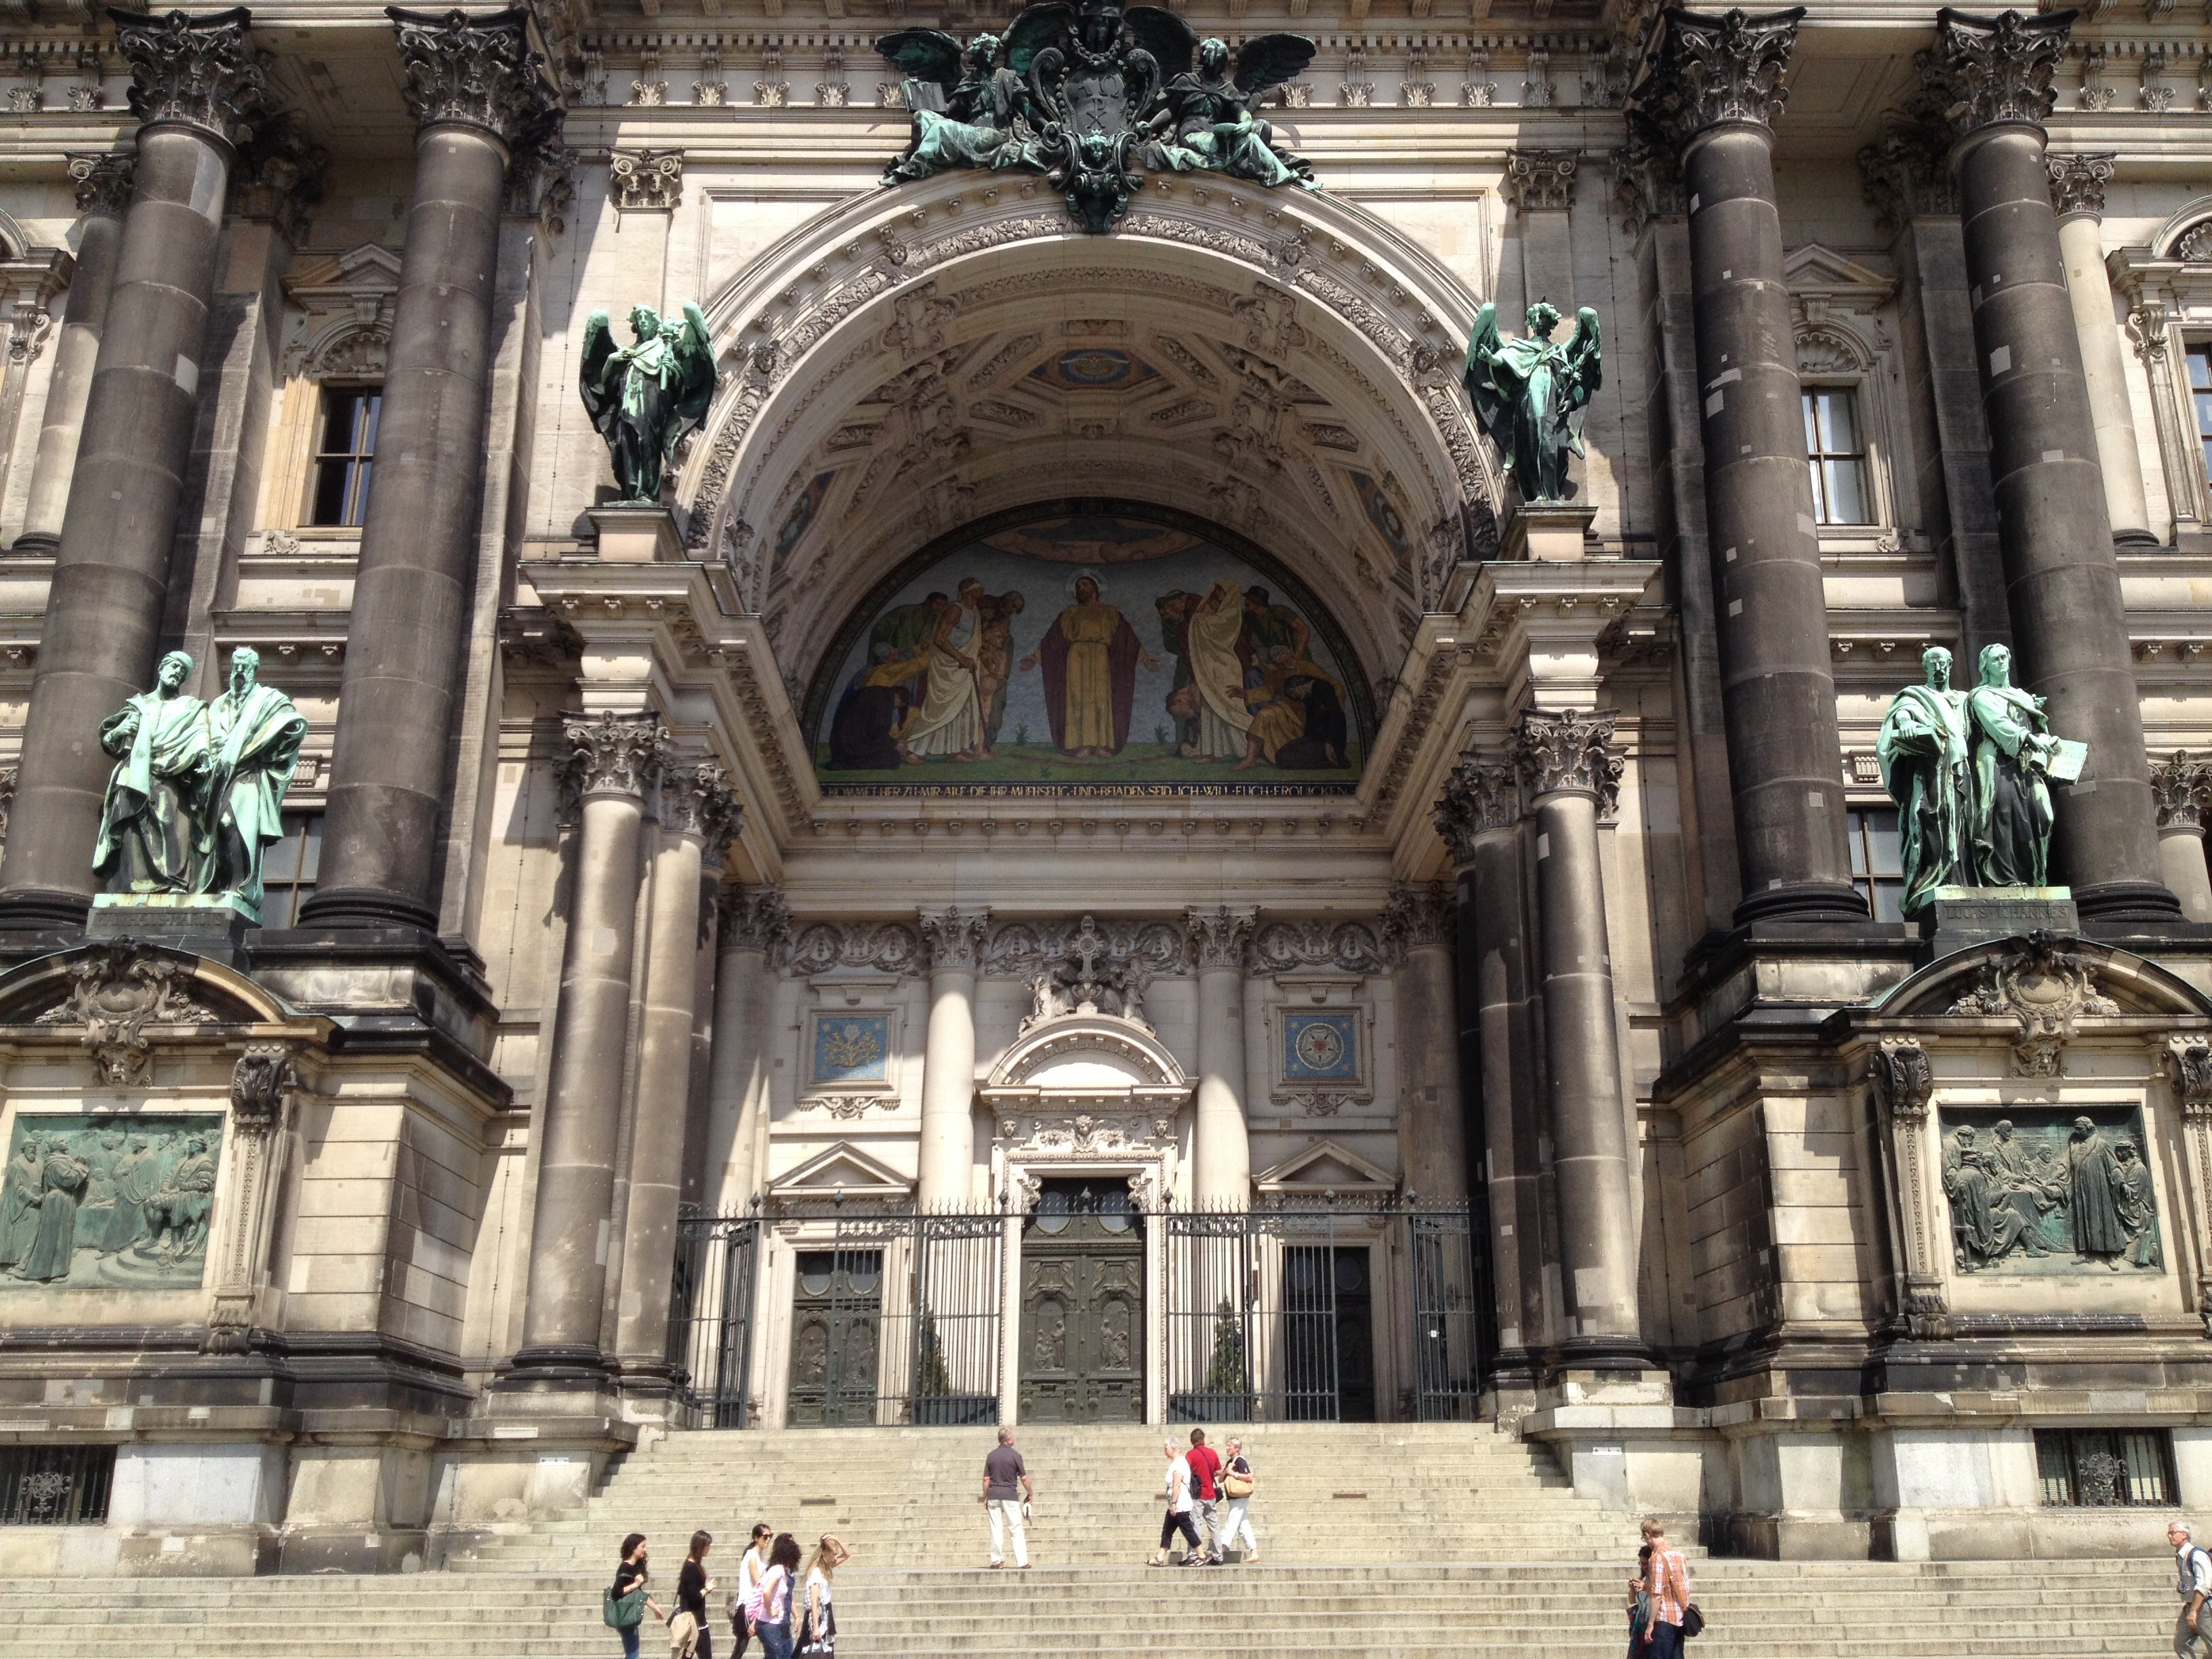
\includegraphics[width=0.8\textwidth]{berlin.jpg}
		\caption{Berlin Cathedral\cite{berlin}}
\end{figure}

Random papers are referenced here\cite{avidanshai} and here\cite{andrewng}. Go check the References page.

Morbi pulvinar turpis at ligula sollicitudin, et finibus nulla vestibulum. Etiam molestie tincidunt molestie. Mauris augue ex, tincidunt non ante eget, ultrices ornare quam\cite{ref1}. Nulla pellentesque fringilla neque, eget facilisis arcu mollis vel. Nulla quam ipsum, vulputate a nisi ut, iaculis tempus ante. Nam efficitur, augue et cursus varius, nisi eros tincidunt ex, porta aliquet massa libero a mauris. Vestibulum finibus, dui sit amet dapibus tincidunt, libero quam venenatis elit, ut porta dui neque a nunc. Donec tincidunt eleifend mauris a luctus. Vivamus eget porttitor metus. Etiam eu porta orci. Suspendisse imperdiet orci sed lobortis vestibulum. Pellentesque sit amet euismod eros.\\

For an ideal gas,
\begin{equation}
    P \cdot V = n \cdot R \cdot T
\end{equation}

\section{Another Section}
\subsection{Another subsection}

Curabitur $P$ and $V$ are the malesuada purus ac orci elementum, ac mollis lectus ornare. Nunc eget nunc non nunc viverra porttitor vel eget nibh. Phasellus nec finibus neque, vitae volutpat purus. Donec vitae sapien dictum, elementum ex eget, iaculis dui. Nulla elementum viverra purus.\\

Here is an image of Berlin Cathedral.

\begin{figure}[H]
		\centering
		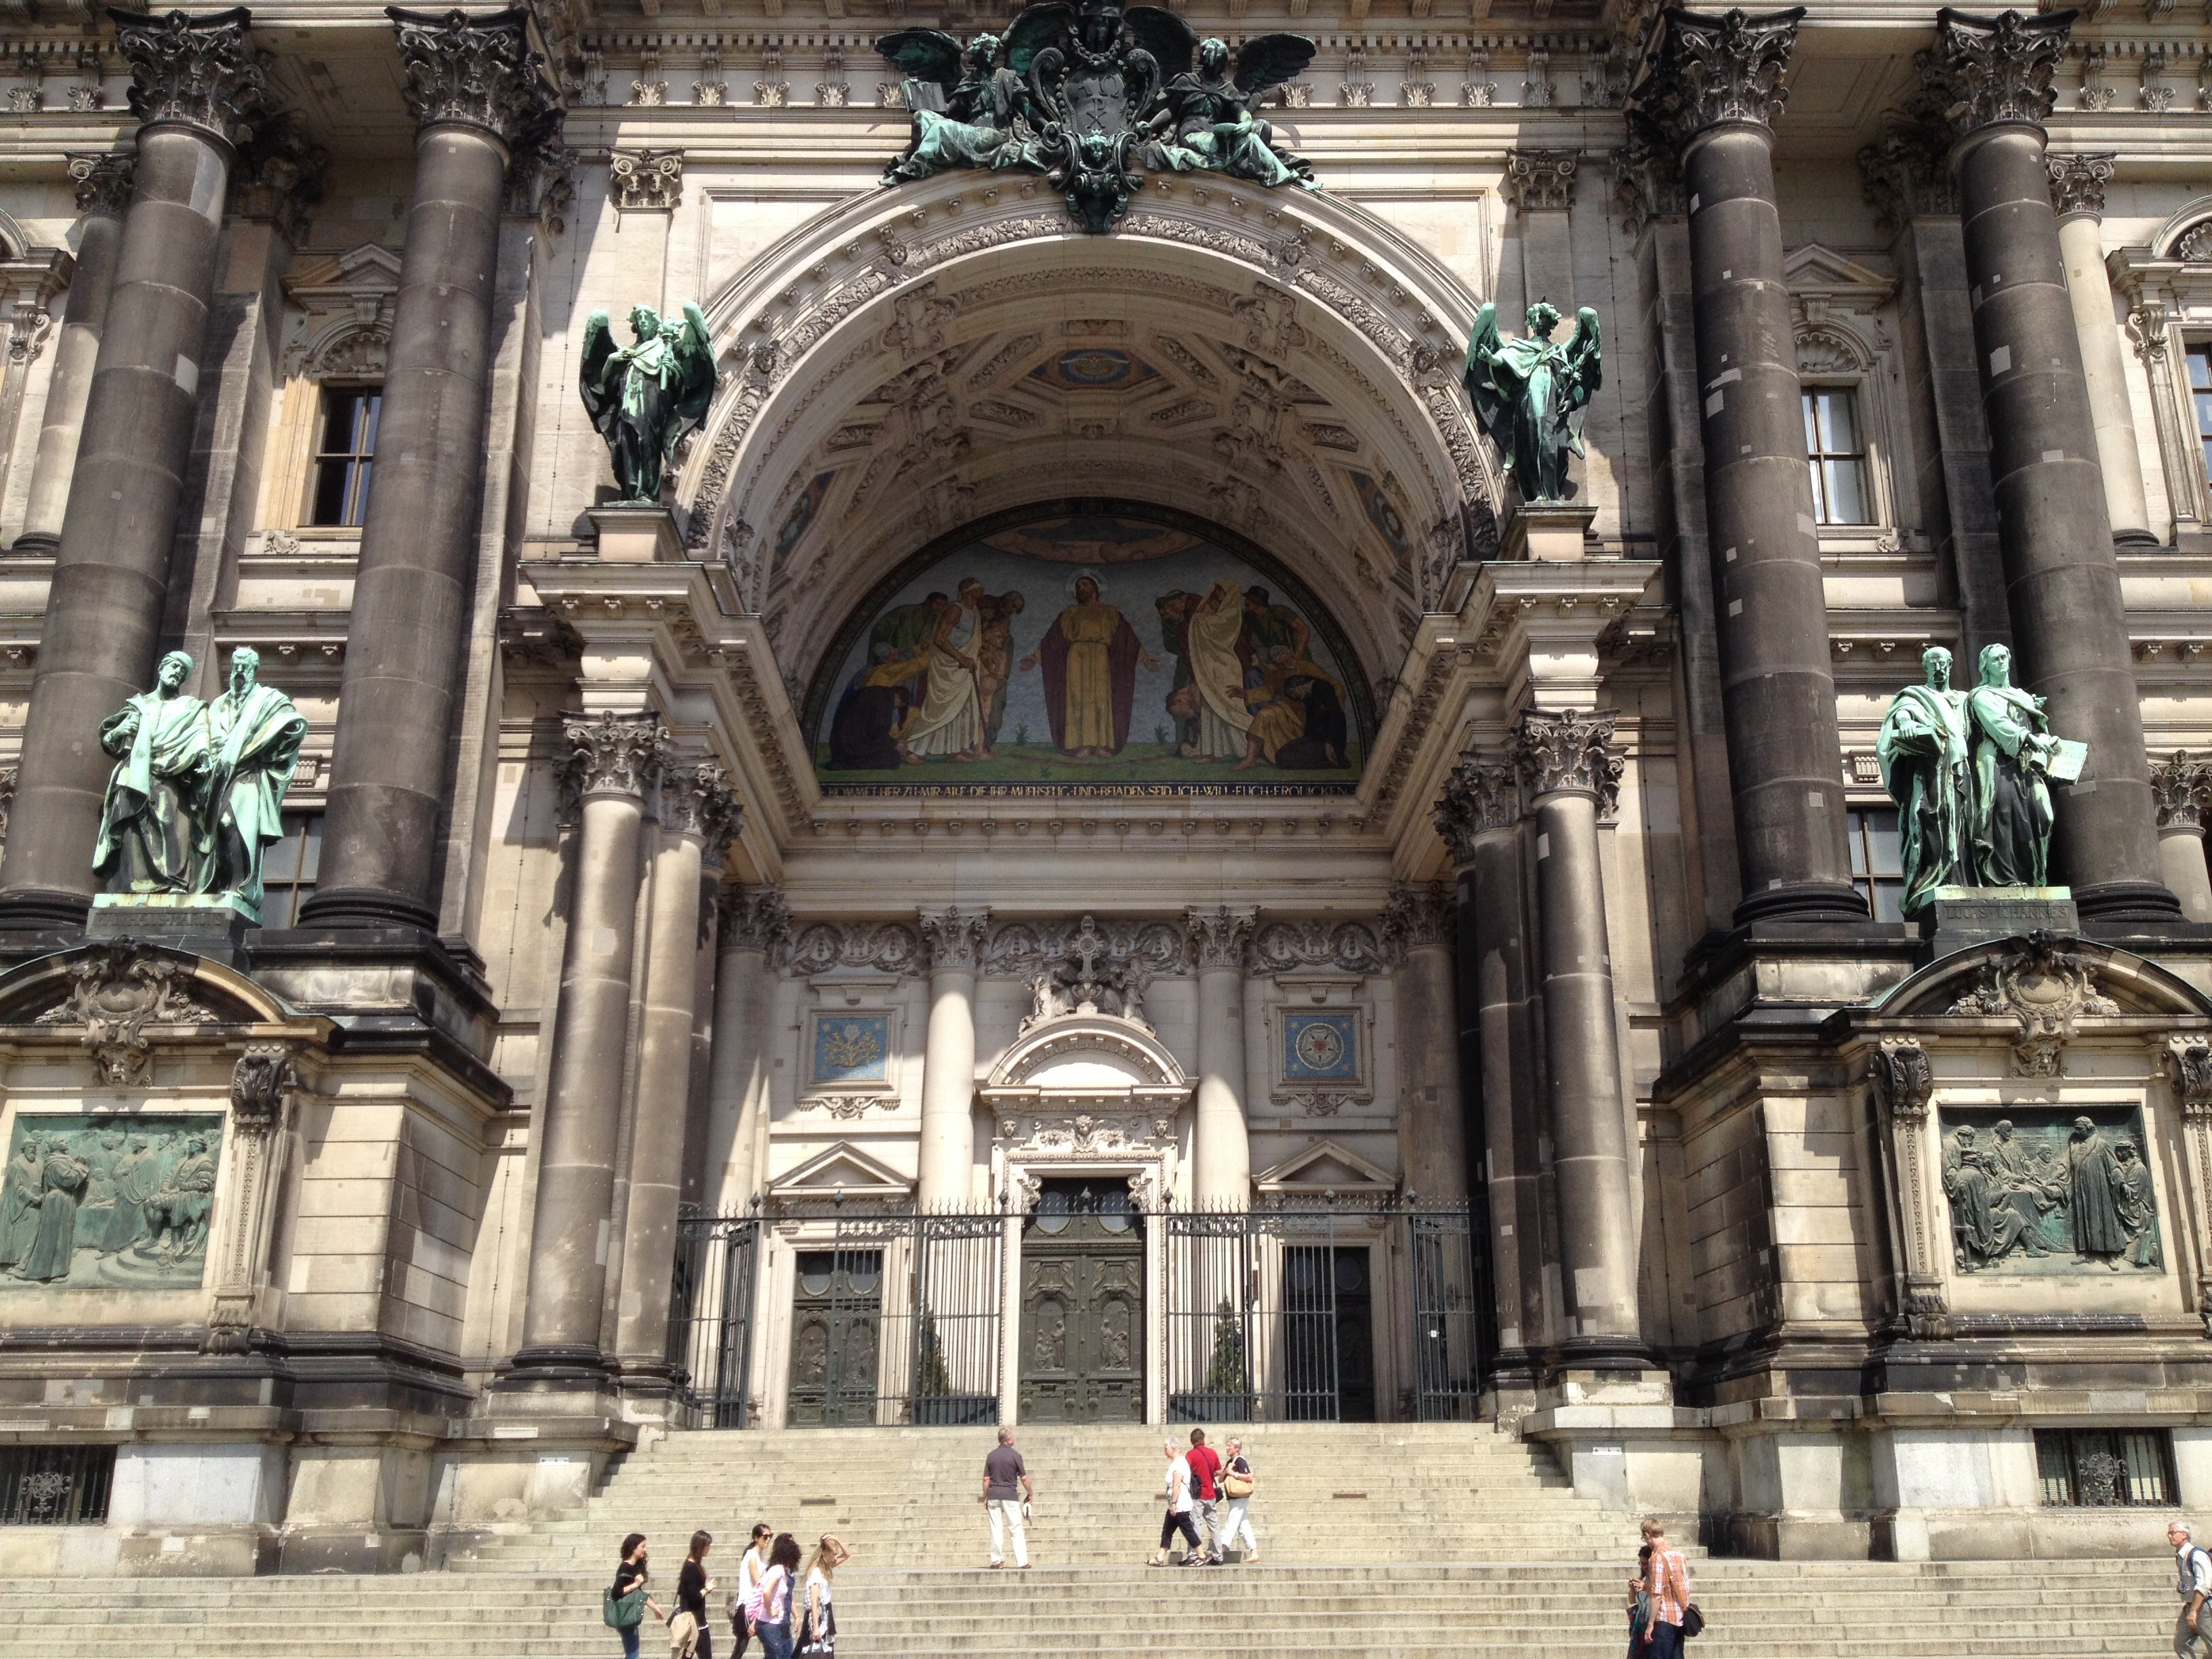
\includegraphics[width=0.8\textwidth]{berlin.jpg}
		\caption{Berlin Cathedral\cite{berlin}}
\end{figure}

Random papers are referenced here\cite{avidanshai} and here\cite{andrewng}. Go check the References page.


\chapter{RELATED WORKS}

\section{A Section}

Lorem ipsum\cite{loremipsum} dolor sit amet, consectetur adipiscing elit. Etiam consectetur libero dui, sit amet rutrum lectus mollis ac. Phasellus mattis augue quis auctor ullamcorper. Sed congue rutrum turpis, sit amet tincidunt erat laoreet ac. Morbi in feugiat erat, sit amet placerat lorem. Quisque cursus gravida nulla, nec pulvinar justo rutrum eget. Aenean et dolor vitae enim congue maximus. Praesent consequat finibus imperdiet. Sed ipsum erat, efficitur vitae urna a, convallis ornare ipsum. Quisque fringilla risus enim, ut elementum dui consectetur eu.

\subsection{Part of a section}

Vivamus sed enim quam. In facilisis consequat eros, id convallis diam congue et. Vivamus sed neque rutrum, gravida urna non, lobortis leo. Curabitur sagittis turpis sit amet dolor blandit lobortis. Fusce ac sem eget libero semper ultrices. Aliquam erat volutpat. Quisque tincidunt mi sapien, eu varius libero lacinia quis. Nullam dictum quam sed scelerisque aliquet. Mauris laoreet est nec dolor pellentesque dignissim. Praesent ac sapien erat. Mauris ut felis sit amet velit convallis cursus quis a tellus. Curabitur efficitur ultricies dui, eget vestibulum arcu venenatis ac. Nulla fermentum dolor a venenatis posuere. Vivamus eu luctus erat.\\

Here is a table attached :
\begin{table}[H]
    \centering
        \begin{tabular}{|c|c|}
        \hline
        $n$ & $F_n$\\
        \hline
        1 & 1 \\
        \hline
        2 & 1 \\
        \hline
        3 & 2 \\
        \hline
        4 & 3 \\
        \hline
        \end{tabular}
    \caption{Fibonacci Table}
\end{table}

Morbi pulvinar turpis at  ligula sollicitudin, et finibus nulla vestibulum. Etiam molestie tincidunt molestie. Mauris augue ex, tincidunt non ante eget, ultrices ornare quam. Nulla pellentesque fringilla neque, eget facilisis arcu mollis vel. Nulla quam ipsum, vulputate a nisi ut, iaculis tempus ante. Nam efficitur, augue et cursus varius, nisi eros tincidunt ex, porta aliquet massa libero a mauris. Vestibulum finibus, dui sit amet dapibus tincidunt, libero quam venenatis elit, ut porta dui neque a nunc. Donec tincidunt eleifend mauris a luctus. Vivamus eget porttitor metus. Etiam eu porta orci. Suspendisse imperdiet orci sed lobortis vestibulum. Pellentesque sit amet euismod eros.\\

For an ideal gas,
\begin{equation}
    P \cdot V = n \cdot R \cdot T
\end{equation}

\section{Another Section}
\subsection{Another subsection}

Curabitur malesuada purus ac orci elementum, ac mollis lectus ornare. Nunc eget nunc non nunc viverra porttitor vel eget nibh. Phasellus nec finibus neque, vitae volutpat purus. Donec vitae sapien dictum, elementum ex eget, iaculis dui. Nulla elementum viverra purus.\\

Here is an image of Berlin Cathedral.

\begin{figure}[H]
		\centering
		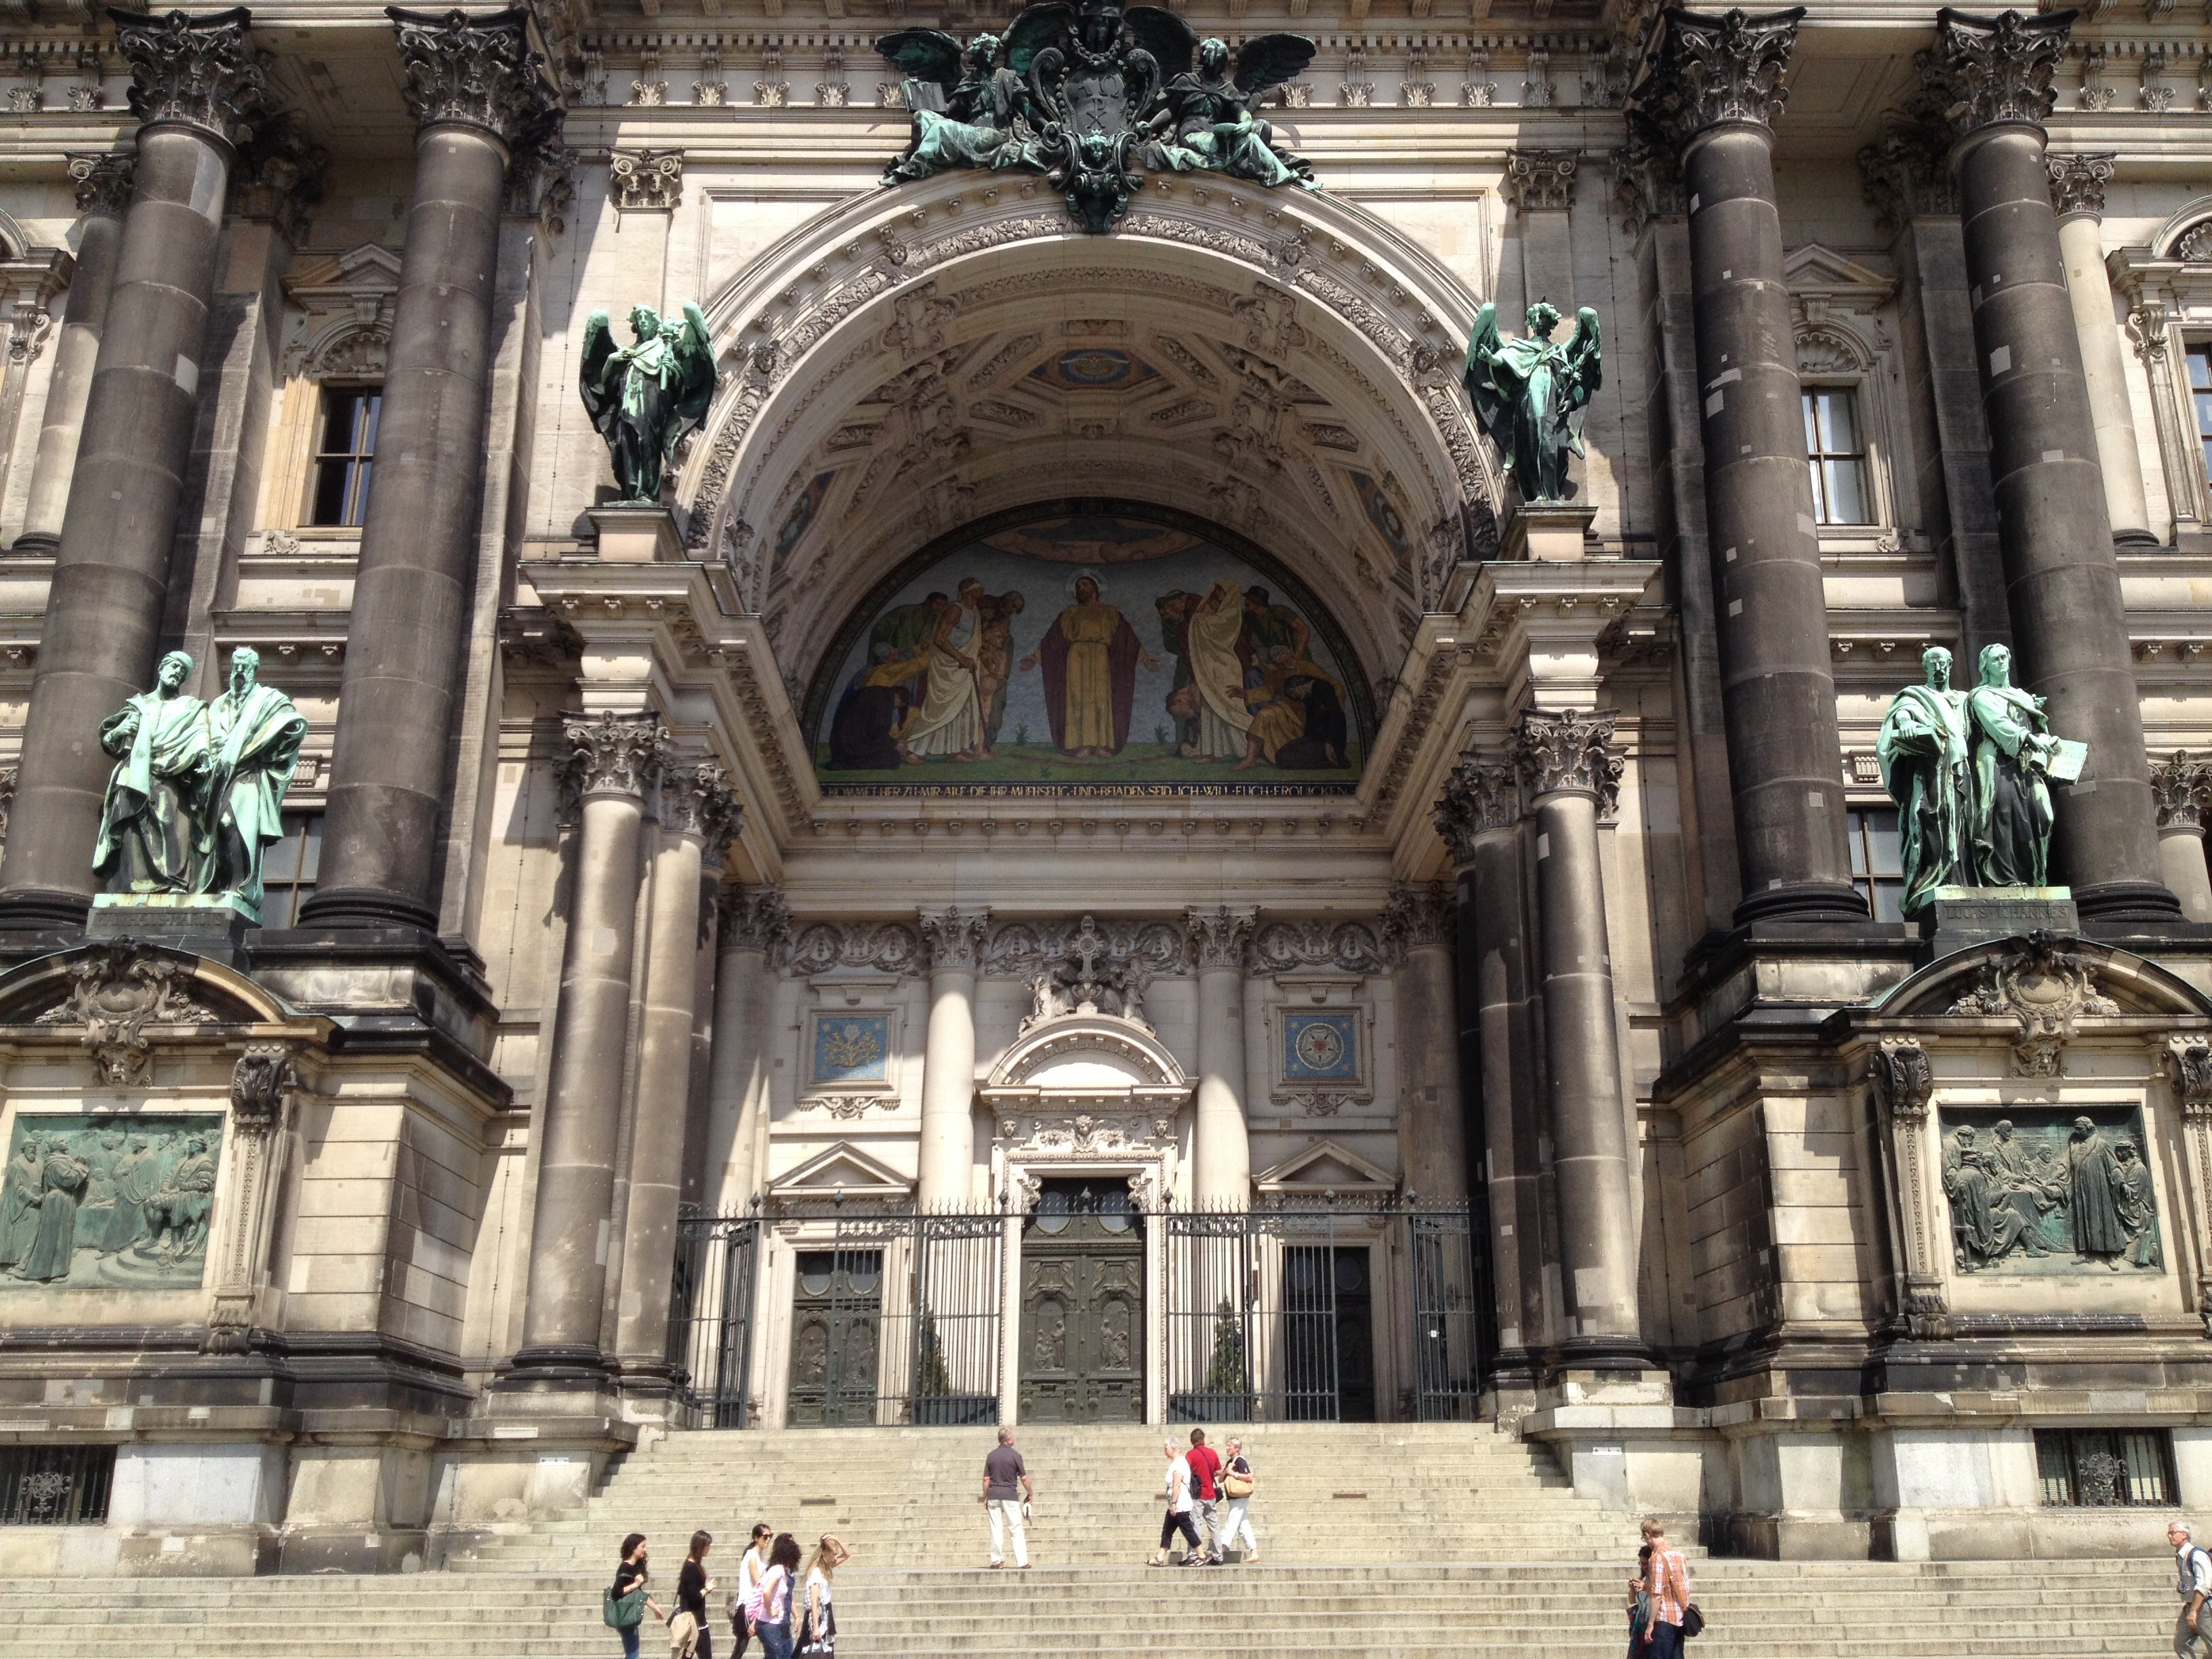
\includegraphics[width=0.8\textwidth]{berlin.jpg}
		\caption{Berlin Cathedral\cite{berlin}}
\end{figure}

\begin{figure}[H]
		\centering
		\includegraphics[width=0.8\textwidth]{images/Pink Minimalist Congratulations Top Seller Instagram Post.png}
		\caption{Congartulations}
\end{figure}
Random papers are referenced here\cite{avidanshai} and here\cite{andrewng}. Go check the References page.



% Appendix and Code Attachments
\fontsize{10pt}{10pt}\selectfont

\begin{appendices}
\chapter{CODE ATTACHMENTS}

\section{Find the Largest Among Three Numbers}

\begin{lstlisting}[language=Python]
# Python program to find the largest number among the three input numbers

# change the values of num1, num2 and num3
# for a different result
num1 = 10
num2 = 14
num3 = 12

# uncomment following lines to take three numbers from user
#num1 = float(input("Enter first number: "))
#num2 = float(input("Enter second number: "))
#num3 = float(input("Enter third number: "))

if (num1 >= num2) and (num1 >= num3):
   largest = num1
elif (num2 >= num1) and (num2 >= num3):
   largest = num2
else:
   largest = num3

print("The largest number between",num1,",",num2,"and",num3,"is",largest)
\end{lstlisting}
\end{appendices}

\fontsize{12pt}{12pt}\selectfont


% Change Bibliography to References
\renewcommand\bibname{BIBILOGRAPHY}
\clearpage
\phantomsection
\addcontentsline{toc}{chapter}{BIBILOGRAPHY}
\printbibliography


\end{document}